\documentclass[10pt,twocolumn,letterpaper]{article}

\usepackage{cvpr}
\usepackage{times}
\usepackage{epsfig}
\usepackage{graphicx}
\usepackage{amsmath}
\usepackage{amssymb}

\usepackage{subfigure}
\usepackage{algorithm}
\usepackage{algorithmic}
\usepackage{mathrsfs}
\usepackage{soul}
\usepackage{multirow}
\usepackage{comment}
\usepackage{tabularx}
\usepackage[tableposition=top]{caption}
\usepackage{pbox}

%\usepackage[sort&compress,square,comma]{natbib}

\usepackage{pgfplots}
\usepackage{pgfplotstable}
\usepackage{filecontents,pgfplots}
\usepackage{tikz}
\usetikzlibrary{shapes,matrix,arrows,decorations.pathmorphing, positioning, calc, decorations.markings}
\usepackage{sci}
\renewcommand{\algorithmicrequire}{\textbf{Input:}}
\renewcommand{\algorithmicensure}{\textbf{Output:}}

\setlength\extrarowheight{3pt}


% Include other packages here, before hyperref.

% If you comment hyperref and then uncomment it, you should delete
% egpaper.aux before re-running latex.  (Or just hit 'q' on the first latex
% run, let it finish, and you should be clear).
\usepackage[pagebackref=true,breaklinks=true,letterpaper=true,colorlinks,bookmarks=false]{hyperref}

%\cvprfinalcopy % *** Uncomment this line for the final submission

\def\cvprPaperID{725} % *** Enter the CVPR Paper ID here
\def\httilde{\mbox{\tt\raisebox{-.5ex}{\symbol{126}}}}

% Pages are numbered in submission mode, and unnumbered in camera-ready
\ifcvprfinal\pagestyle{empty}\fi
\begin{document}

%%%%%%%%% TITLE
\title{Supplementary Material for Paper\\``Deep Relative Attributes''}

\author{First Author\\
Institution1\\
Institution1 address\\
{\tt\small firstauthor@i1.org}
% For a paper whose authors are all at the same institution,
% omit the following lines up until the closing ``}''.
% Additional authors and addresses can be added with ``\and'',
% just like the second author.
% To save space, use either the email address or home page, not both
\and
Second Author\\
Institution2\\
First line of institution2 address\\
{\tt\small secondauthor@i2.org}
}

\maketitle
%\thispagestyle{empty}

%%%%%%%%% ABSTRACT

%%%%%%%%% CONTENT
% \section{Implementation Details}
% \subsection{Efficient Implementation}
% In section 3.2 of the main paper we have describe the main 
\section{Optimization Details}
For training, we use stochastic gradient descent with RMSProp \cite{Tieleman2012} updates and mini-batches of size 32 (16 pair of images). We set the learning rate for all experiments to $10^{-4}$ (for all parameters both the feature learning and extraction layers and the ranking layer), initially, then RMSProp changes the learning rates according to its algorithm. We have also used weight decay ($\ell_2$ norm regularization), with a fixed $0.005$ multiplier.

\section{Results}
%Due to lack of space in the main paper,
% We still had space left in the paper, better not to write this
Here, we show a more comprehensive set of results, some of which overlap with the ones in the paper.

\subsection{Quantitative Results}

Here we present the mean accuracy of correct ordering of pairs on various datasets. Table \ref{tab:osr} shows the results of OSR dataset, table \ref{tab:pubfig} shows the results on PubFig dataset, table \ref{tab:lfw} shows the results of LFW10 dataset, table \ref{tab:zap1} shows the results of Zappos50k-1 dataset and table \ref{tab:zap2} shows the results of Zappos50k-2 dataset.
These tables not only include a comparison of our results with previous methods, but also show the mean and standard deviation of our results over 3 different runs.

%%%%%%%%%%%%%%%%%%%%%% OSR RESULTS %%%%%%%%%%%%%%%%%%%%%
\begin{table*}[t!]
\caption{Results for the OSR dataset}
\centering
\resizebox{2\columnwidth}{!}{
\begin{tabular}{l| c | c | c | c | c | c | c }
\textbf{Method} & \textbf{Natural} & \textbf{Open} &  \textbf{Perspective} & \textbf{Large Size} & \textbf{Diag} & \textbf{ClsDepth} & \textbf{Mean}\\ \hline
 Relative Attributes~\cite{parikh2011} &  95.03 & 90.77 & 86.73 & 86.23 & 86.50 & 87.53 & 88.80 \\
 Relative Forest~\cite{Li2013} & 95.24 & 92.39 & 87.58 & 88.34 & 89.34 & 89.54 & 90.41 \\
 Fine-grained Comparison~\cite{Yu2014} & 95.70 & 94.10 & 90.43 & 91.10 & 92.43 & 90.47 & 92.37 \\
 VGG16-fc7 (baseline) & 97.98 & 87.82 & 89.01 & 88.25 & 89.91 & 90.70 & 90.61 \\ \hline
 \multirow{2}{*}{RankNet (ours)} & 97.76  & 94.48  & 92.37  & 92.70  & 95.14  & 91.44  & \textbf{93.98}  \\
        & ($\pm$ 0.25)                  & ($\pm$ 0.90)                  & ($\pm$ 0.34)             & ($\pm$ 1.01)              & ($\pm$ 0.26)              & ($\pm$ 2.69)        & ($\pm$ 0.35) \\                   
 \hline
 %RankNet (ours) & 97.76 & 94.48 & 92.37 & 92.70 & 95.14 & 91.44 & \textbf{93.98}
\end{tabular}}
\label{tab:osr}
\end{table*}
%%%%%%%%%%%%%%%%%%%%%%%%%%%%%%%%%%%%%%%%%%%%%%%%%%%%%%%%%


%%%%%%%%%%%%%%%%%%%%%% PUBFIG RESULTS %%%%%%%%%%%%%%%%%%%
\begin{table*}[t!]
\caption{Results for the PubFig dataset}
\centering
\resizebox{2\columnwidth}{!}{
\begin{tabular}{l|c|c|c|c|c|c|c|c|c|c|c|c}
 \textbf{Method} & \textbf{Male} & \textbf{White} & \textbf{Young} & \textbf{Smiling} & \textbf{Chubby} & \textbf{Forehead} & \textbf{Eyebrow} & \textbf{Eye} & \textbf{Nose} & \textbf{Lip} & \textbf{Face} & \textbf{Mean}  \\ \hline
 Relative Attributes~\cite{parikh2011} & 81.80 & 76.97 & 83.20 & 79.90 & 76.27 & 87.60 & 79.87 & 81.67 & 77.40 & 79.17 & 82.33 & 80.53 \\ 
 Relative Forest~\cite{Li2013} & 85.33 & 82.59 & 84.41 & 83.36 & 78.97 & 88.83 & 81.84 & 83.15 & 80.43 & 81.87 & 86.31 & 83.37 \\
 Fine-grained Comparison~\cite{Yu2014} & 91.77 & 87.43 & 91.87 & 87.00 & 87.37 & 94.00 & 89.83 & 91.40 & 89.07 & 90.43 & 86.70 & \textbf{89.72} \\
 VGG16-fc7 (baseline) & 80.84 & 73.39 & 79.41 & 76.23 & 74.69 & 80.52 & 75.38 & 77.78 & 76.15 & 78.14 & 80.01 & 77.50 \\
 \hline
 % & \pbox{20cm}{\centering 90.10\\($\pm$ 1.05)} & 89.49 ($\pm$ 0.59) & 89.83 ($\pm$ 0.37) & 88.62 ($\pm$ 1.59) & 88.72 ($\pm$ 0.75) & 9.33 ($\pm$ 0.80) & 88.13 ($\pm$ 1.83) & 86.94 ($\pm$ 3.36) & 86.30 ($\pm$ 1.60) & 89.79 ($\pm$ 0.45) & 92.71 ($\pm$ 1.87) & \textbf{89.36 ($\pm$ 0.57)} \\
 \multirow{2}{*}{RankNet (ours)} & 90.10 & 89.49 & 89.83 & 88.62 & 88.72 & 92.33 & 88.13 & 86.94 & 86.30 & 89.79 & 92.71 & \textbf{89.36} \\
                                 & ($\pm$ 1.05) & ($\pm$ 0.59) & ($\pm$ 0.37) & ($\pm$ 1.59) & ($\pm$ 0.75) & ($\pm$ 0.80) &  ($\pm$ 1.83) & ($\pm$ 3.36) & ($\pm$ 1.60) & ($\pm$ 0.45) & ($\pm$ 1.87) & ($\pm$ 0.57) \\
 \hline
\end{tabular}}
\label{tab:pubfig}
\end{table*}
%%%%%%%%%%%%%%%%%%%%%%%%%%%%%%%%%%%%%%%%%%%%%%%%%%%%%%%%

%%%%%%%%%%%%%%%%%%%%%%% LFW10 RESULTS %%%%%%%%%%%%%%%%%%
\begin{table*}
\caption{Results for the LFW10 dataset}
\centering
\resizebox{2\columnwidth}{!}{
\begin{tabular}{l|c|c|c|c|c|c|c|c|c|c|c}
 \textbf{Method} & \textbf{Bald} & \textbf{DkHair} & \textbf{Eyes} & \textbf{GdLook} & \textbf{Mascu.} & \textbf{Mouth} & \textbf{Smile} & \textbf{Teeth} & \textbf{FrHead} & \textbf{Young} & \textbf{Mean} \\ \hline
 Fine-grained Comparison~\cite{Li2013} & 67.9 & 73.6 & 49.6 & 64.7 & 70.1 & 53.4 & 59.7 & 53.5 & 65.6 & 66.2 & 62.4  \\
 Relative Attributes~\cite{parikh2011} & 70.4 & 75.7 & 52.6 & 68.4 & 71.3 & 55.0 & 54.6 & 56.0 & 64.5 & 65.8 & 63.4 \\
 Relative Parts~\cite{Sandeep_2014_CVPR} & 71.8 & 80.5 & 90.5 & 77.6 & 67.0 & 77.6 & 81.3 & 76.2 & 80.2 & 82.4 & 78.5 \\
 Global + HOG~\cite{vermaexploring} & 78.8 & 72.4 & 70.7 & 67.6 & 84.5 & 67.8 & 67.4 & 71.7 & 79.3 & 68.4 & 72.9 \\
 VGG16-fc7 (baseline) & 70.44 & 69.14 & 59.40 & 59.75 & 84.48 & 56.04 & 57.63 & 57.85 & 59.38 & 70.36 & 64.45 \\
 %RankNet (ours) & 81.27  & 88.92 & 91.98  & 72.03  & 95.40  & 89.04 & 84.75  & 89.33   & 84.11  & 73.35  & \textbf{85.02 }\\
 \hline
 \multirow{2}{*}{RankNet (ours)} & 81.27 & 88.92 & 91.98 & 72.03 & 95.40 & 89.04 & 84.75 & 89.33 & 84.11 & 73.35 & \textbf{85.02} \\
                                 & ($\pm$ 1.47) & ($\pm$ 1.63) & ($\pm$ 2.42) & ($\pm$ 1.25) & ($\pm$ 1.52) & ($\pm$ 2.18) & ($\pm$ 0.28) & ($\pm$ 0.47) & ($\pm$ 2.77) & ($\pm$ 1.13) & ($\pm$ 0.59) \\
 \hline
\end{tabular}}
\label{tab:lfw}
\end{table*}
%%%%%%%%%%%%%%%%%%%%%%%%%%%%%%%%%%%%%%%%%%%%%%%%%%%%%%%%


%%%%%%%%%%%%%%%%%%%%%% Zap50K-1 RESULTS %%%%%%%%%%%%%%%%
\begin{table*}
\caption{Results for the UT-Zap50K-1 (coarser) dataset}
\centering
\resizebox{1.5\columnwidth}{!}{
\begin{tabular}{l|c|c|c|c|c}
 \textbf{Method} & \textbf{Open} & \textbf{Pointy} & \textbf{Sporty} & \textbf{Comfort} & \textbf{Mean} \\ \hline
 Relative Attributes~\cite{parikh2011} & 87.77 & 89.37 & 91.20 & 89.93 & 89.57 \\
 Fine-grained Comparison~\cite{Yu2014} & 90.67 & 90.83 & 92.67 & 92.37 & 91.64 \\
 VGG16-fc7 (baseline) & 62.33 & 59.57 & 61.33 & 61.00 & 61.08 \\
 %RankNet (ours) & 93.00  & 92.11  & 95.56  & 93.22 & \textbf{93.47 } \\
 \hline
 \multirow{2}{*}{RankNet (ours)} & 93.00 & 92.11 & 95.56 & 93.22 & \textbf{93.47}\\
                                 & ($\pm$ 1.15) & ($\pm$ 1.58) & ($\pm$ 1.26) & ($\pm$ 2.41) & ($\pm$ 0.59)\\
 \hline
\end{tabular}}
\label{tab:zap1}
\end{table*}
%%%%%%%%%%%%%%%%%%%%%%%%%%%%%%%%%%%%%%%%%%%%%%%%%%%%%%%%


%%%%%%%%%%%%%%%%%%%%%% Zap50K-2 RESULTS %%%%%%%%%%%%%%%%
\begin{table*}
\caption{Results for the UT-Zap50K-2 (fine-grained) dataset}
\centering
\resizebox{1.5\columnwidth}{!}{
\begin{tabular}{l|c|c|c|c|c}
 \textbf{Method} & \textbf{Open} & \textbf{Pointy} & \textbf{Sporty} & \textbf{Comfort} & \textbf{Mean} \\ \hline
 Relative Attributes~\cite{parikh2011} & 60.18 & 59.56 & 62.70 & 64.04 & 61.62  \\
 Fine-grained Comparison~\cite{Yu2014} & 74.91 & 63.74 & 64.54 & 62.51 & 66.43  \\
 LocalPair + ML + HOG~\cite{vermaexploring} & 76.2 & 65.3 & 64.8 & 63.6 & 67.5 \\
 VGG16-fc7 (baseline) & 52.55 & 52.65 & 51.52 & 53.01 & 52.43 \\
 %RankNet (ours) & 70.48  & 66.64  & 67.81 & 64.32  & \textbf{67.31 } \\
 \hline
 \multirow{2}{*}{RankNet (ours)} & 71.21 & 66.64 & 67.81 & 65.88 & \textbf{67.88} \\
                                 & ($\pm$ 1.50) & ($\pm$ 1.81) & ($\pm$ 0.84) & ($\pm$ 1.92) & ($\pm$ 0.83)\\
 \hline
\end{tabular}}
\label{tab:zap2}
\end{table*}
%%%%%%%%%%%%%%%%%%%%%%%%%%%%%%%%%%%%%%%%%%%%%%%%%%%%%%%%

\subsection{Qualitative Results}
For qualitative analysis of our proposed method we use \cite{saliency}, as described in section 4.5 of the paper, to visualize the saliency maps of each attributes. We have plotted saliency maps for a set of test pairs from LFW10 dataset in Figures \ref{sal.lfw.bald}-\ref{sal.lfw.young}.
We see from this set of figures, that the network has learned to correctly localize different attributes.


\begin{figure*}
    \centering
    \begin{subfigure}
        \centering
        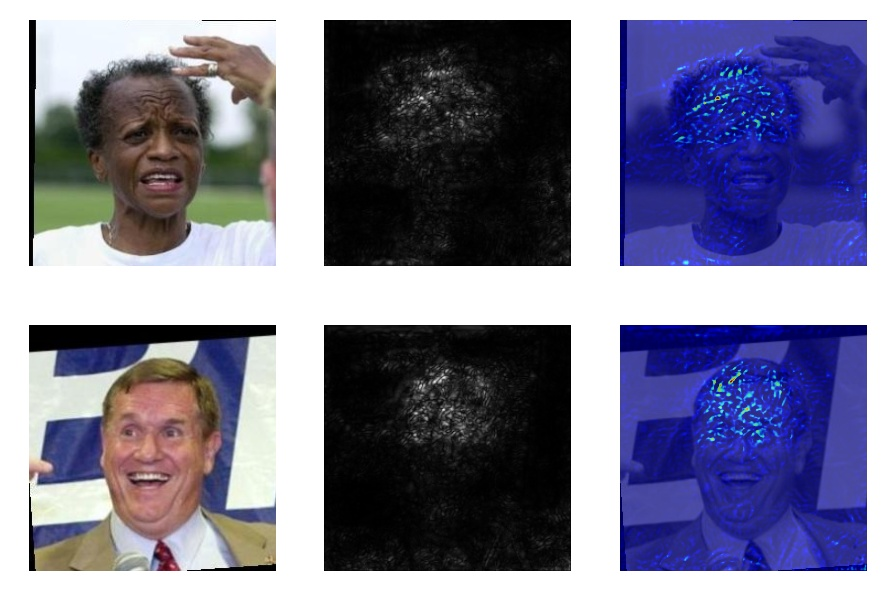
\includegraphics[width=7cm]{saliency-new/LFW/bald-1}
    \end{subfigure}
    \begin{subfigure}
        \centering
        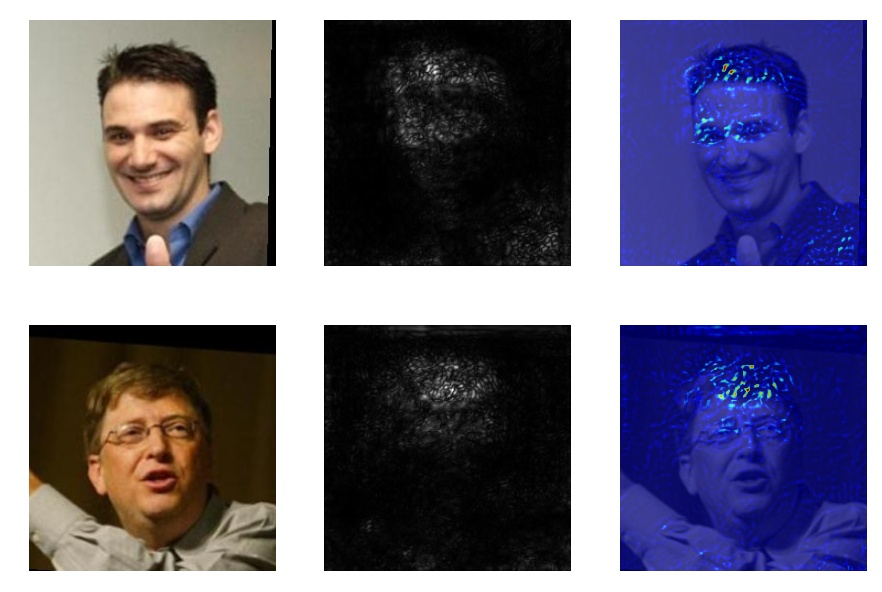
\includegraphics[width=7cm]{saliency-new/LFW/bald-2}
    \end{subfigure}
    \begin{subfigure}
        \centering
        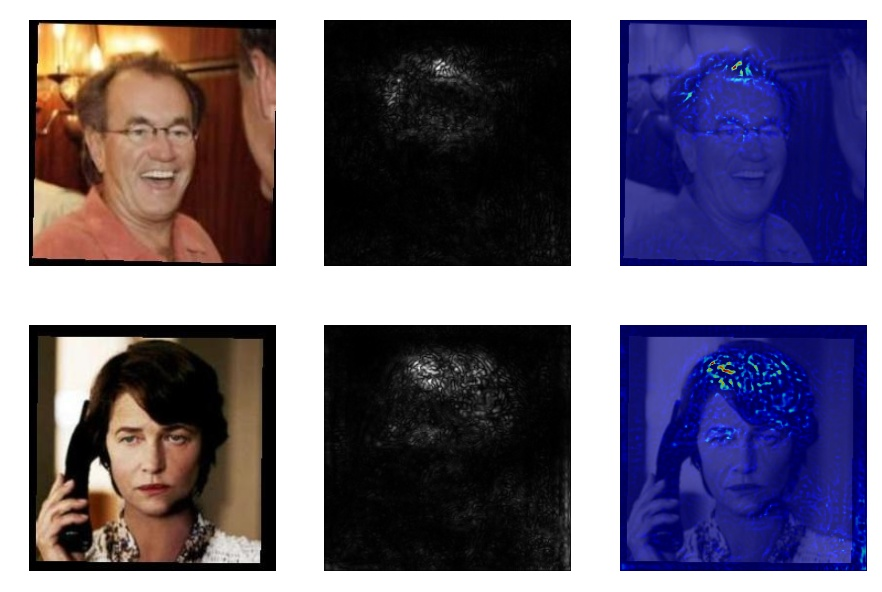
\includegraphics[width=7cm]{saliency-new/LFW/bald-4}
    \end{subfigure}
    \begin{subfigure}
        \centering
        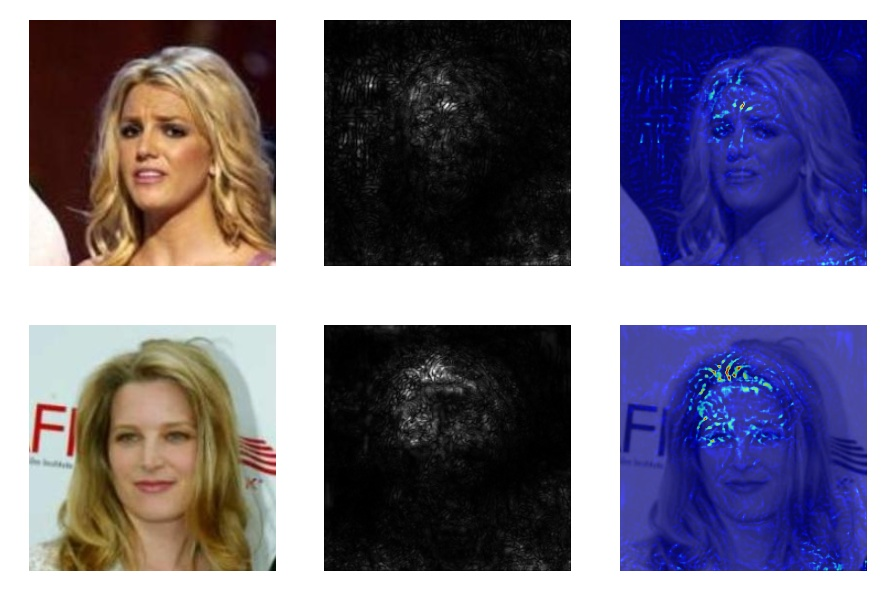
\includegraphics[width=7cm]{saliency-new/LFW/bald-6}
    \end{subfigure}
    
    \caption{Saliency maps obtained from the network. Visualizing a localization for "Bald Head" relative attribute on the LFW10 dataset.}
    \label{sal.lfw.bald}
\end{figure*}

\begin{figure*}
    \centering
    \begin{subfigure}
        \centering
        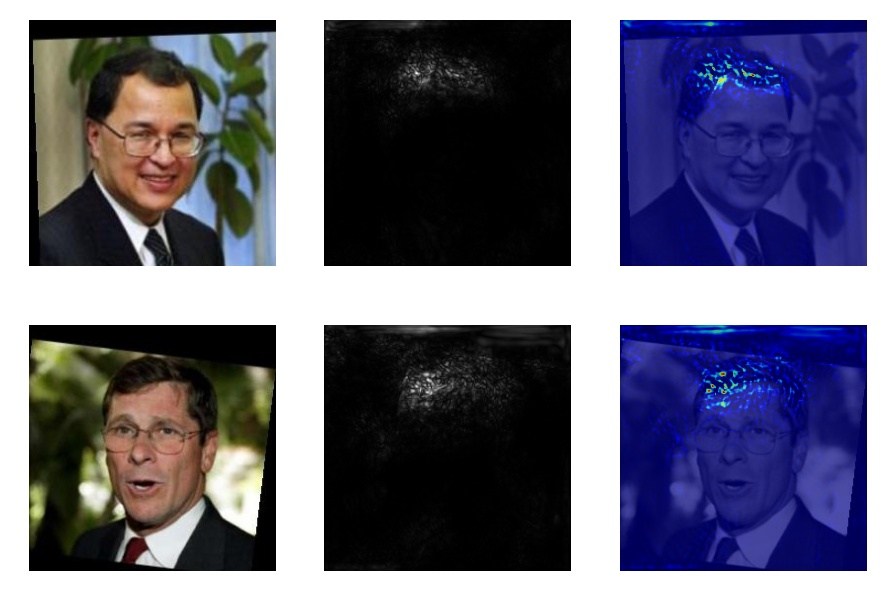
\includegraphics[width=7cm]{saliency-new/LFW/darkhair-1}
    \end{subfigure}
    \begin{subfigure}
        \centering
        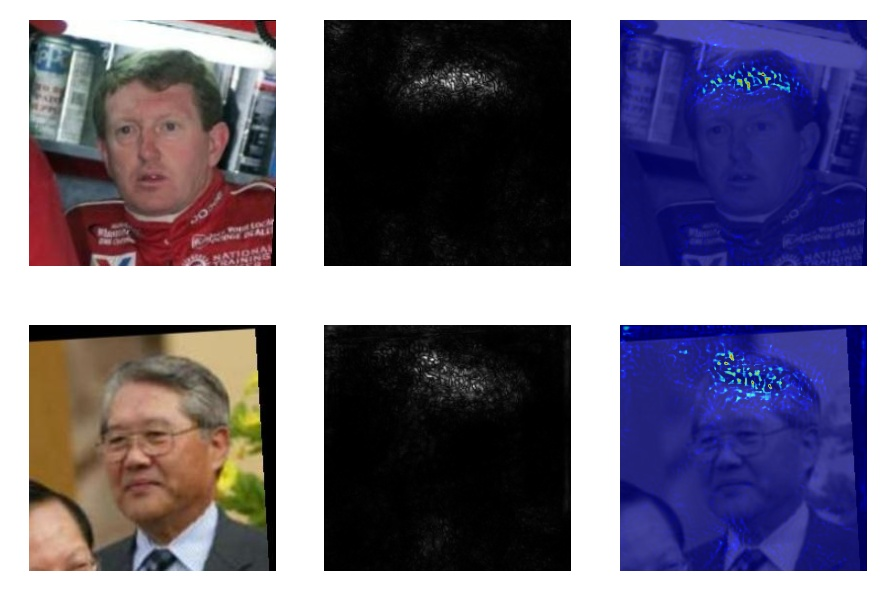
\includegraphics[width=7cm]{saliency-new/LFW/darkhair-2}
    \end{subfigure}
    \begin{subfigure}
        \centering
        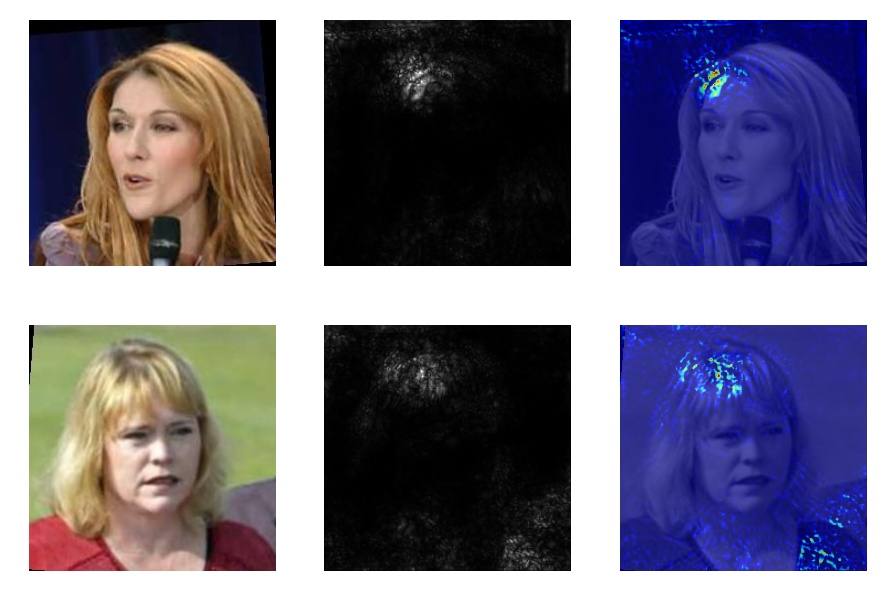
\includegraphics[width=7cm]{saliency-new/LFW/darkhair-4}
    \end{subfigure}
    \begin{subfigure}
        \centering
        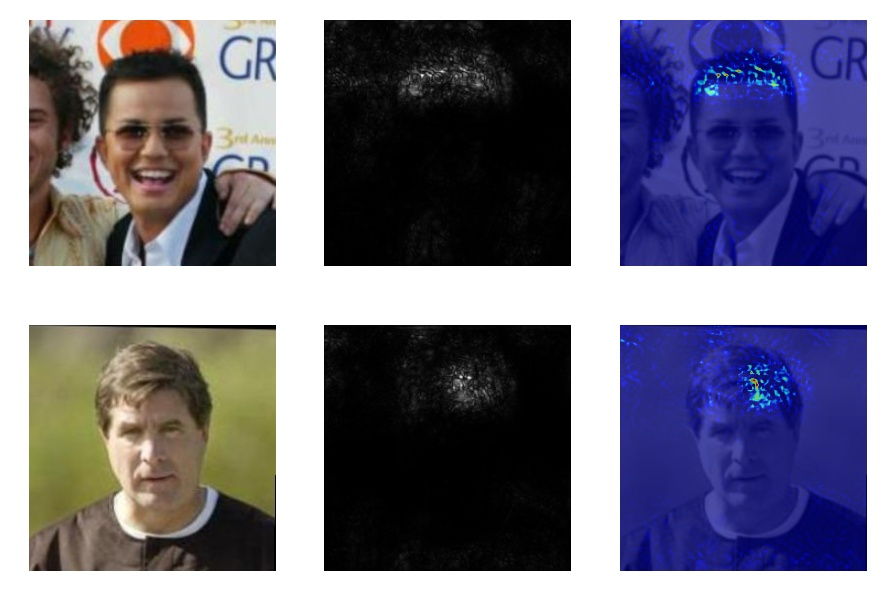
\includegraphics[width=7cm]{saliency-new/LFW/darkhair-6}
    \end{subfigure}
    
    \caption{Saliency maps obtained from the network. Visualizing a localization for "Dark Hair" relative attribute on the LFW10 dataset.}
    \label{sal.lfw.harkhair}
\end{figure*}

\begin{figure*}
    \centering
    \begin{subfigure}
        \centering
        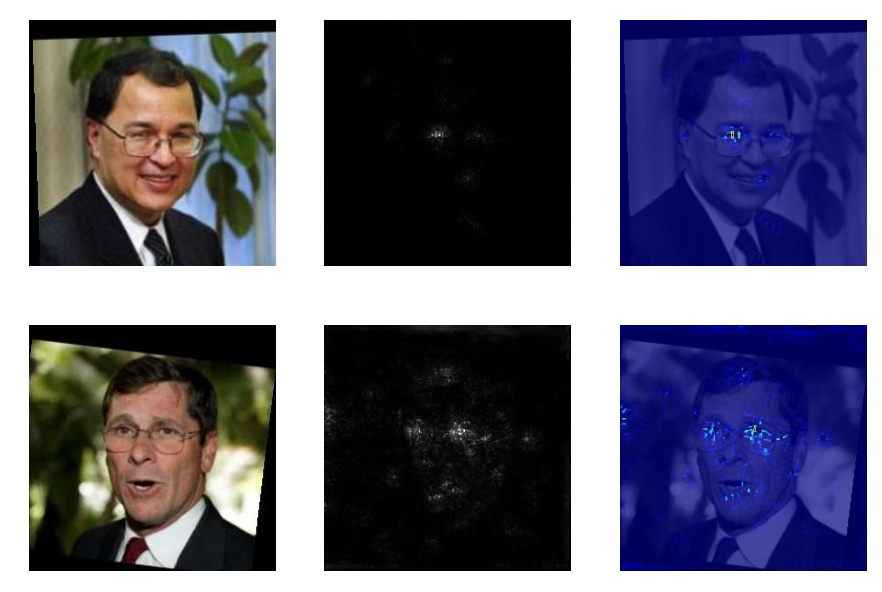
\includegraphics[width=7cm]{saliency-new/LFW/eyesopen-1}
    \end{subfigure}
    \begin{subfigure}
        \centering
        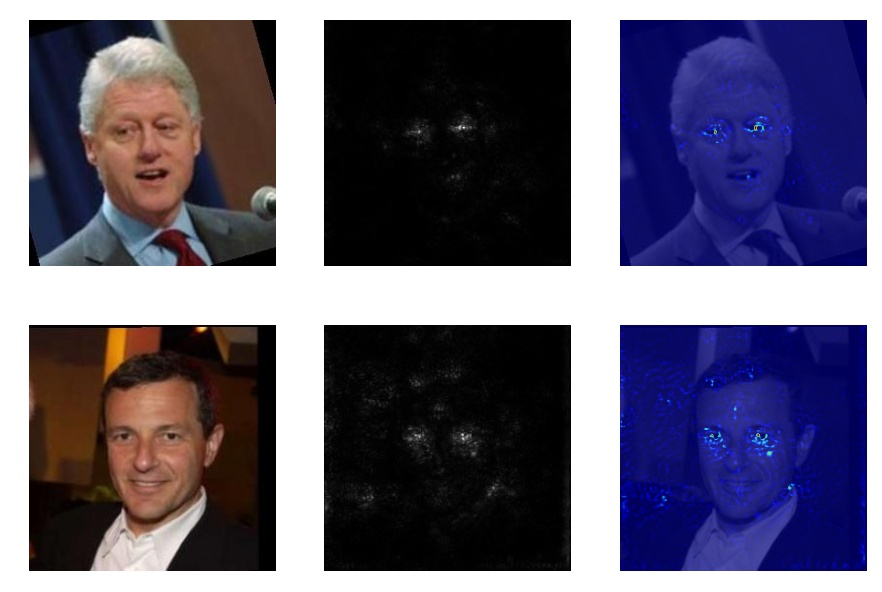
\includegraphics[width=7cm]{saliency-new/LFW/eyesopen-2}
    \end{subfigure}
    \begin{subfigure}
        \centering
        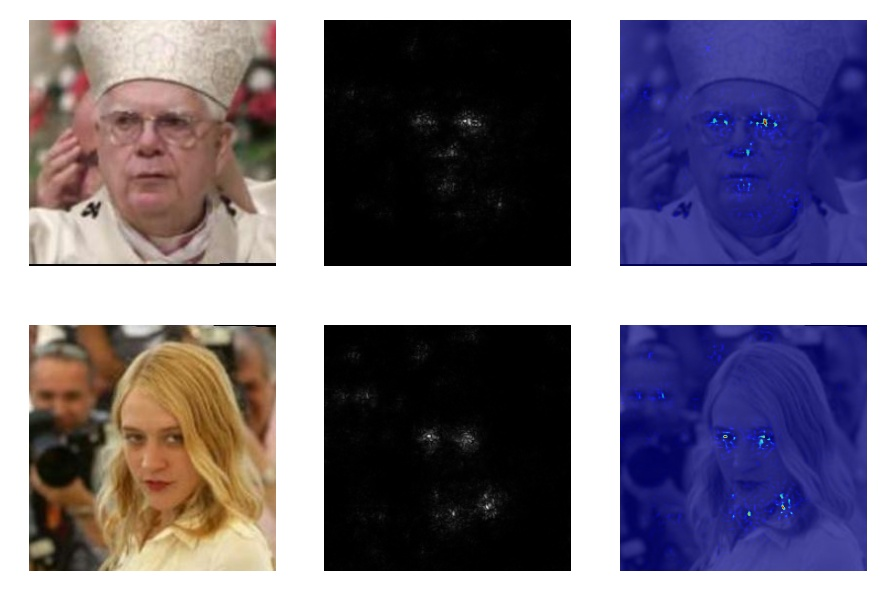
\includegraphics[width=7cm]{saliency-new/LFW/eyesopen-4}
    \end{subfigure}
    \begin{subfigure}
        \centering
        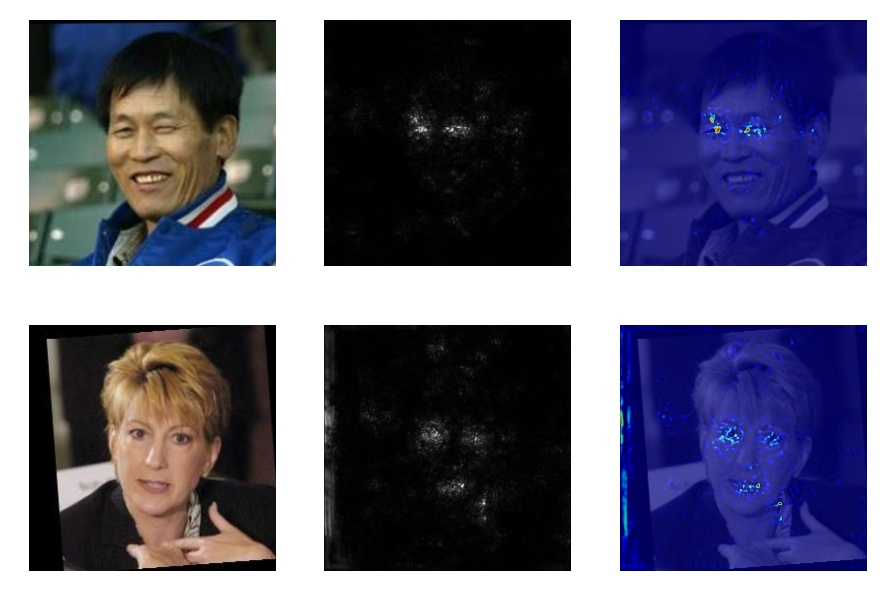
\includegraphics[width=7cm]{saliency-new/LFW/eyesopen-6}
    \end{subfigure}
    
    \caption{Saliency maps obtained from the network. Visualizing a localization for "Eyes Open" relative attribute on the LFW10 dataset.}
    \label{sal.lfw.eyesopen}
\end{figure*}

\begin{figure*}
    \centering
    \begin{subfigure}
        \centering
        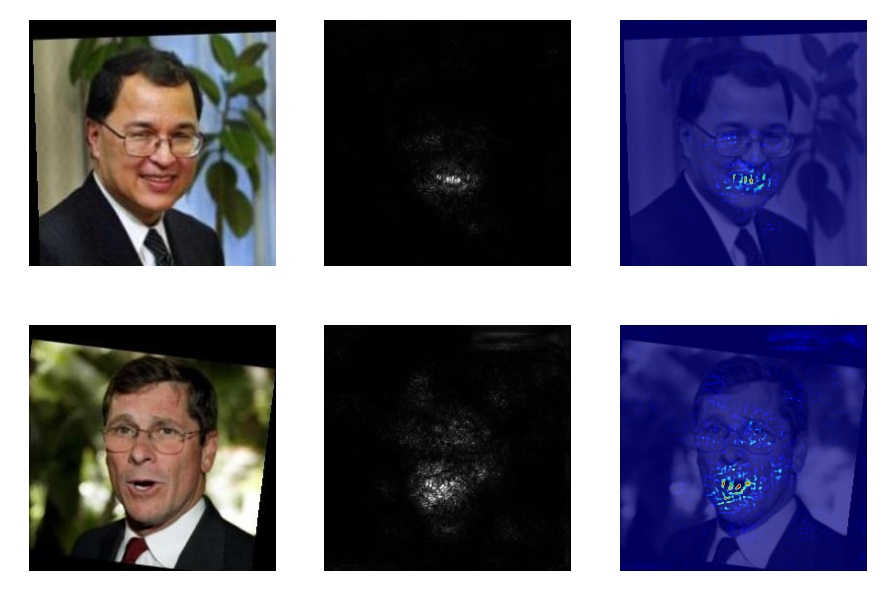
\includegraphics[width=7cm]{saliency-new/LFW/mouthopen-1}
    \end{subfigure}
    \begin{subfigure}
        \centering
        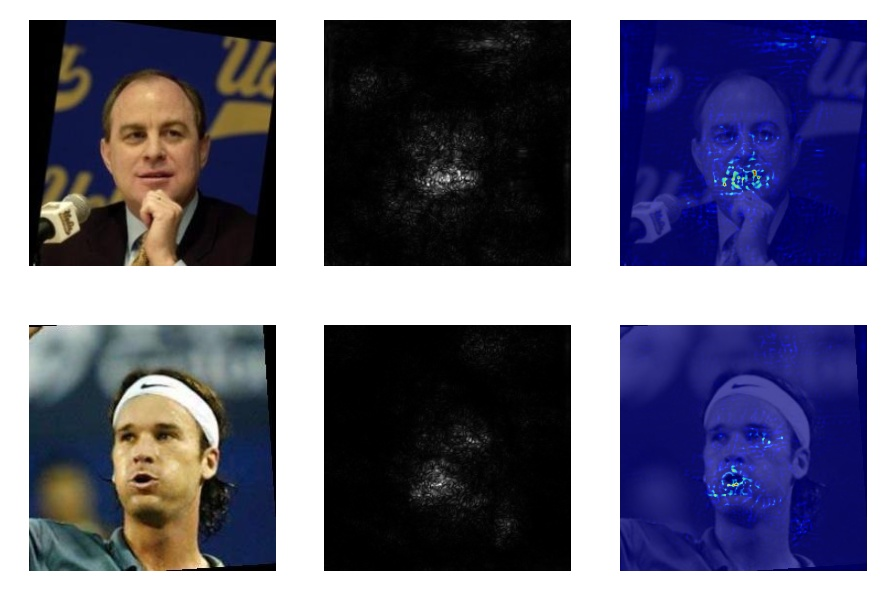
\includegraphics[width=7cm]{saliency-new/LFW/mouthopen-2}
    \end{subfigure}
    \begin{subfigure}
        \centering
        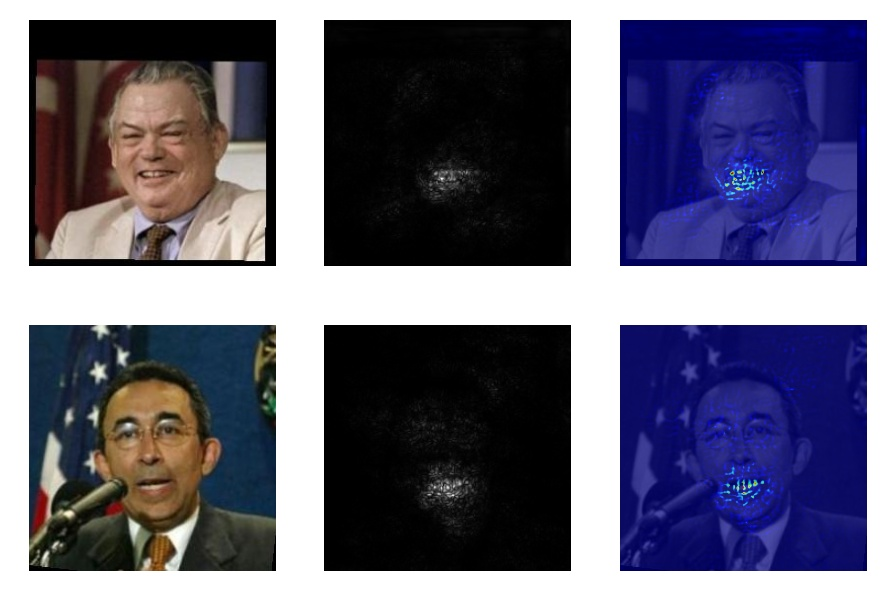
\includegraphics[width=7cm]{saliency-new/LFW/mouthopen-4}
    \end{subfigure}
    \begin{subfigure}
        \centering
        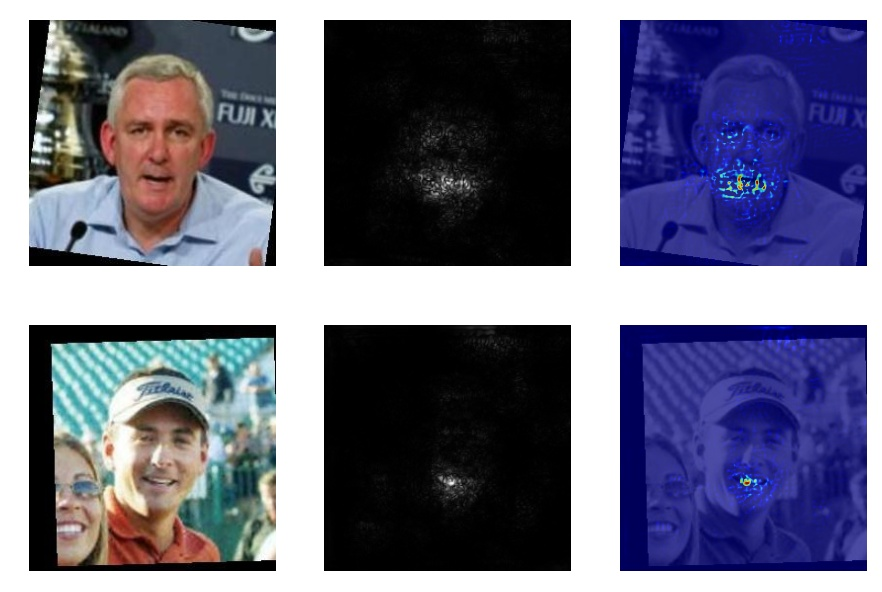
\includegraphics[width=7cm]{saliency-new/LFW/mouthopen-6}
    \end{subfigure}
    
    \caption{Saliency maps obtained from the network. Visualizing a localization for "Mouth Open" relative attribute on the LFW10 dataset.}
    \label{sal.lfw.mouthopen}
\end{figure*}

\begin{figure*}
    \centering
    \begin{subfigure}
        \centering
        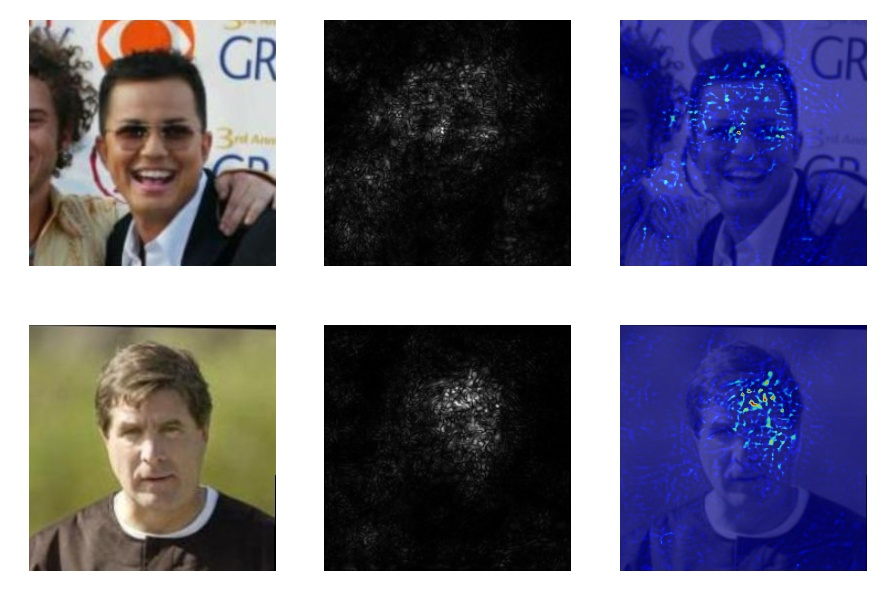
\includegraphics[width=7cm]{saliency-new/LFW/vforehead-1}
    \end{subfigure}
    \begin{subfigure}
        \centering
        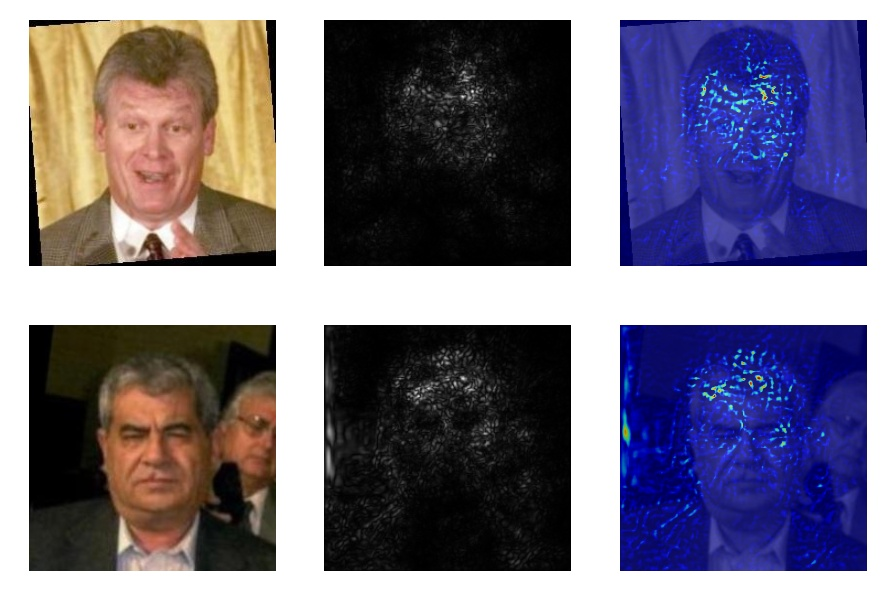
\includegraphics[width=7cm]{saliency-new/LFW/vforehead-2}
    \end{subfigure}
    \begin{subfigure}
        \centering
        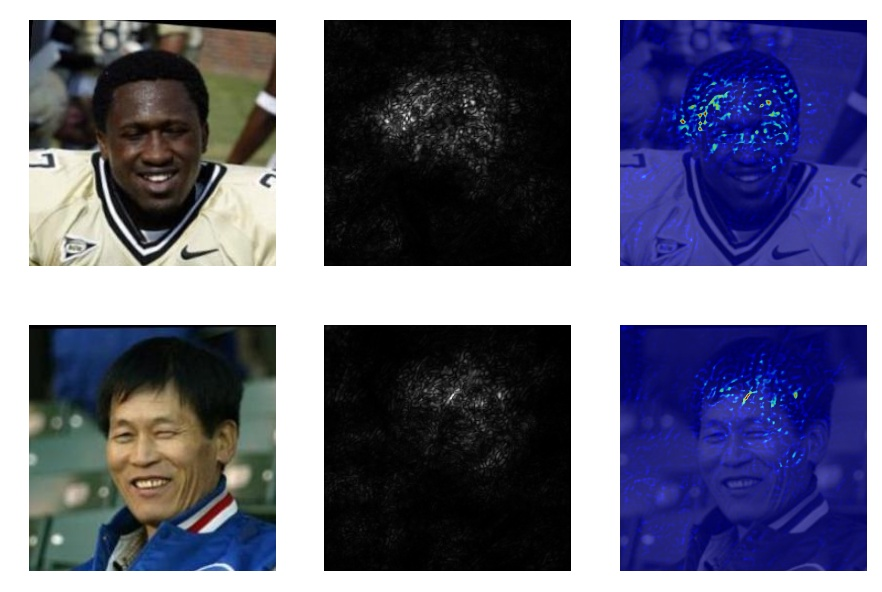
\includegraphics[width=7cm]{saliency-new/LFW/vforehead-4}
    \end{subfigure}
    \begin{subfigure}
        \centering
        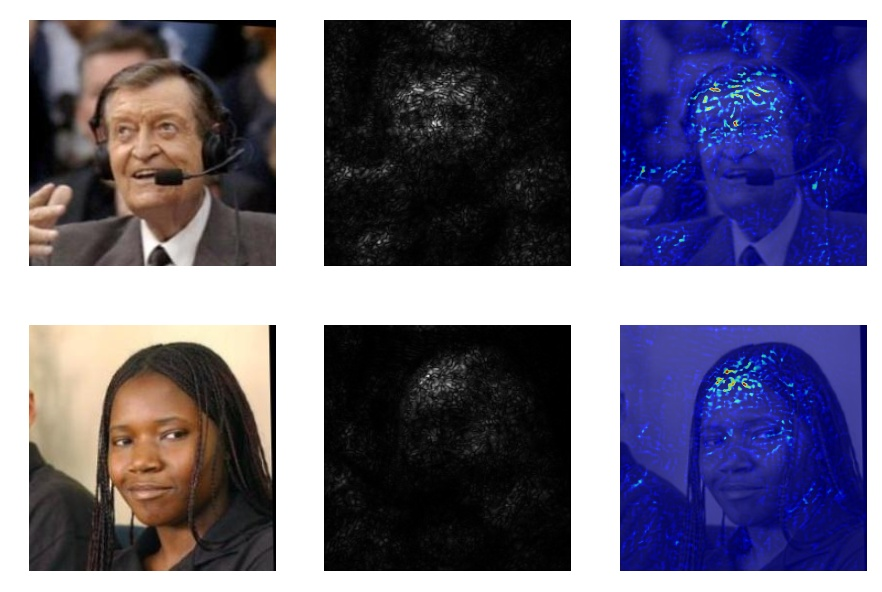
\includegraphics[width=7cm]{saliency-new/LFW/vforehead-5}
    \end{subfigure}
    
    \caption{Saliency maps obtained from the network. Visualizing a localization for "Visible Forehead" relative attribute on the LFW10 dataset.}
    \label{sal.lfw.vforehead}
\end{figure*}

\begin{figure*}
    \centering
    \begin{subfigure}
        \centering
        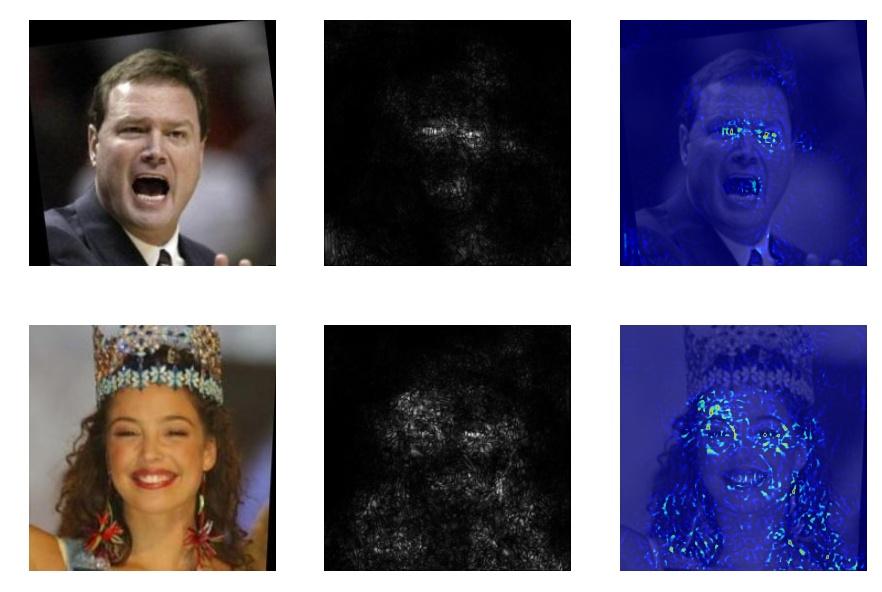
\includegraphics[width=7cm]{saliency-new/LFW/young-1}
    \end{subfigure}
    \begin{subfigure}
        \centering
        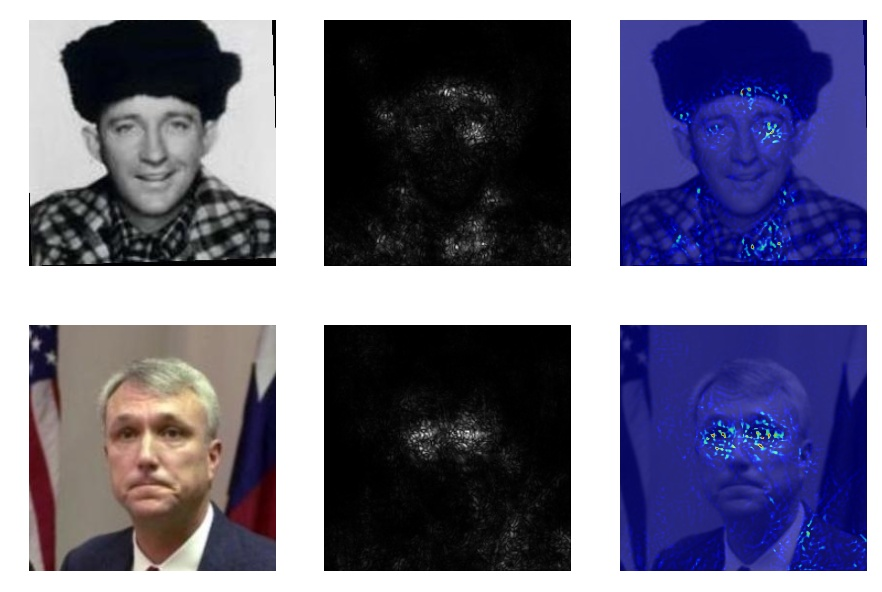
\includegraphics[width=7cm]{saliency-new/LFW/young-2}
    \end{subfigure}
    \begin{subfigure}
        \centering
        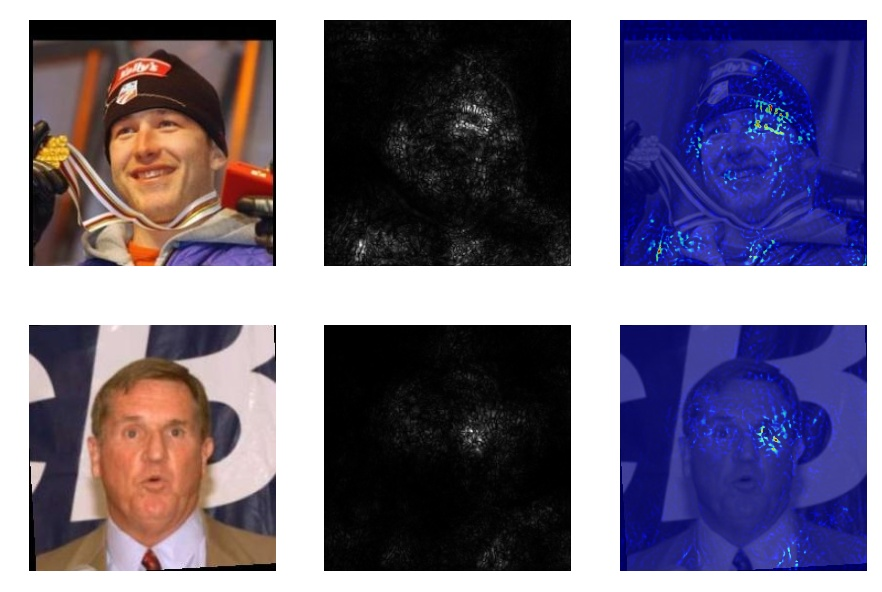
\includegraphics[width=7cm]{saliency-new/LFW/young-4}
    \end{subfigure}
    \begin{subfigure}
        \centering
        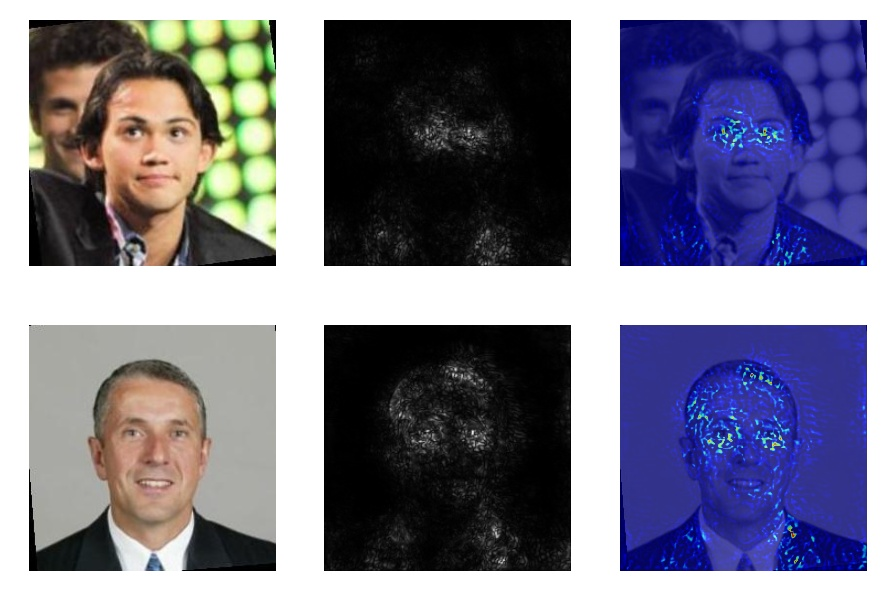
\includegraphics[width=7cm]{saliency-new/LFW/young-6}
    \end{subfigure}
    
    \caption{Saliency maps obtained from the network. Visualizing a localization for "Young" relative attribute on the LFW10 dataset.}
    \label{sal.lfw.young}
\end{figure*}

\subsection{Features}
% The feature extraction part of the network is a fine-tuned version of the original VGG 16 network.
To show the effectiveness of fine-tuning on the features, we compare the feature representations of the pre-trained VGG-16 network and the fine-tuned network. For each network, we extract the fc7 features of images and then project these feature representations in to 2-D plane using the t-SNE method~\cite{van2008visualizing}. This way we can visually represent and compare the feature representations of each network.
We can see that the fine-tuning has made the features much more appropriate for the task of ranking.

\begin{figure*}
    \centering
    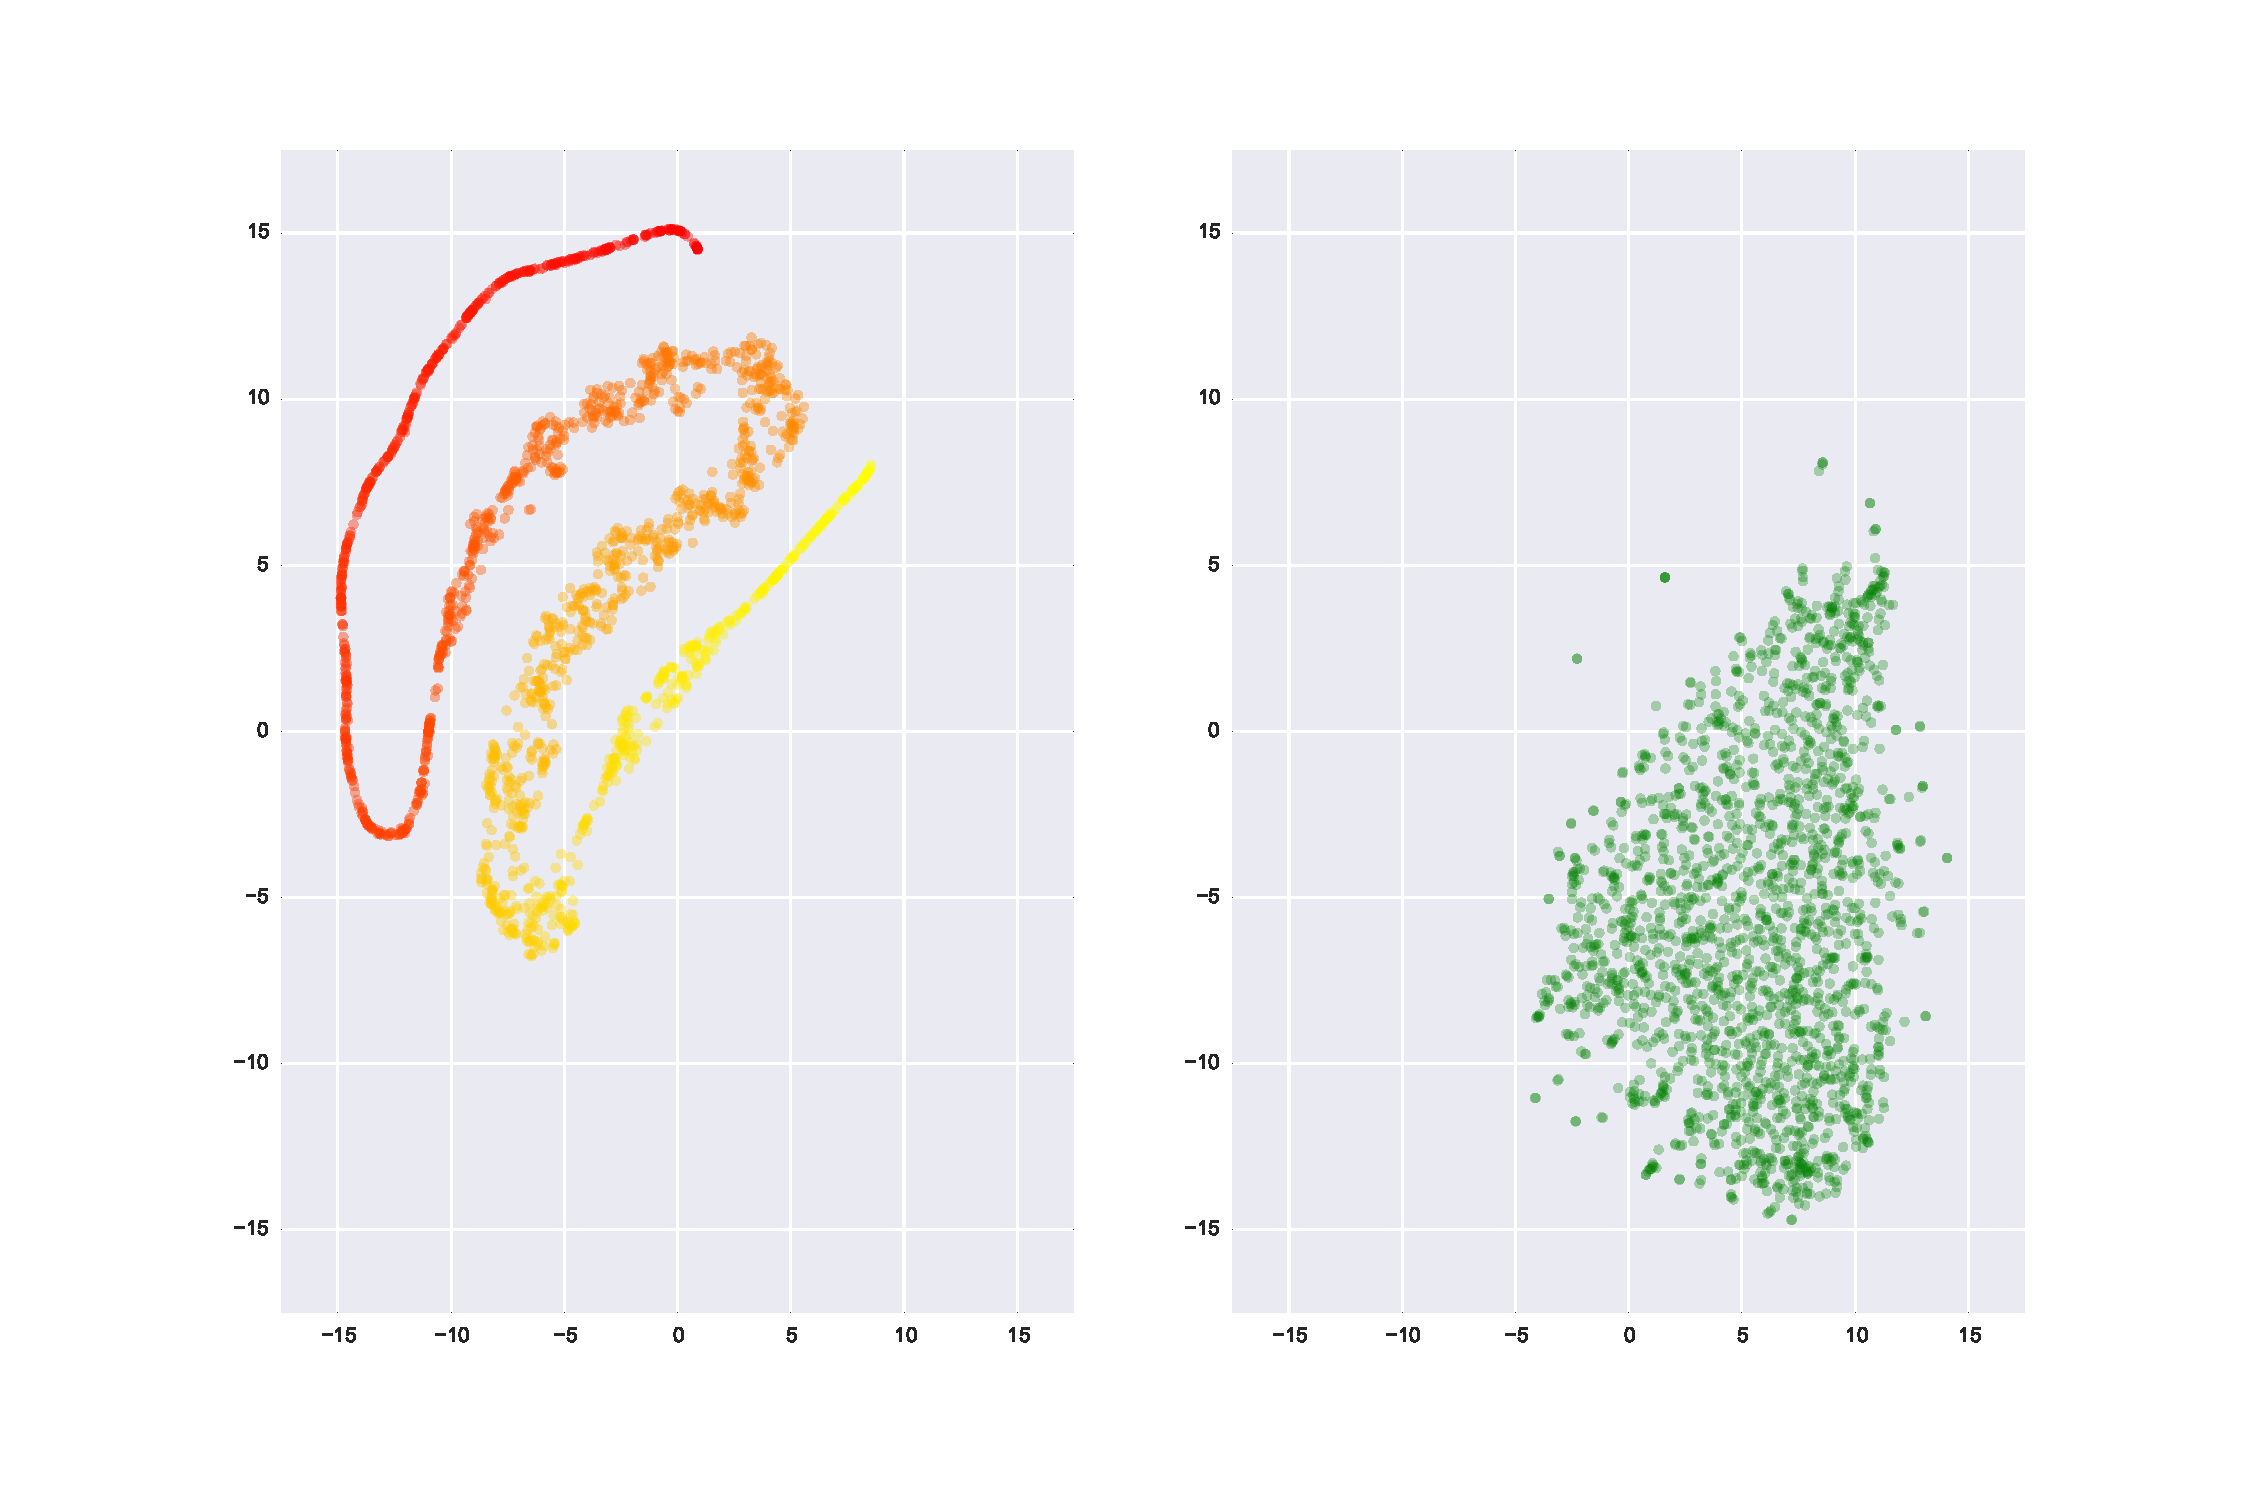
\includegraphics[width=18cm]{att0.pdf}
    \caption{2-D projection of image features for the attribute \textit{Bald Head} of the LFW10 dataset. Figure on the right represent the projection of features from the VGG-16 network. Figure on the left represents the 2-D projections of the image features from RankNet. The change in color reflects the change in the ranking strength of the attribute.}
    \label{fig:tsne_lfw_att0}
\end{figure*}

\begin{figure*}
    \centering
    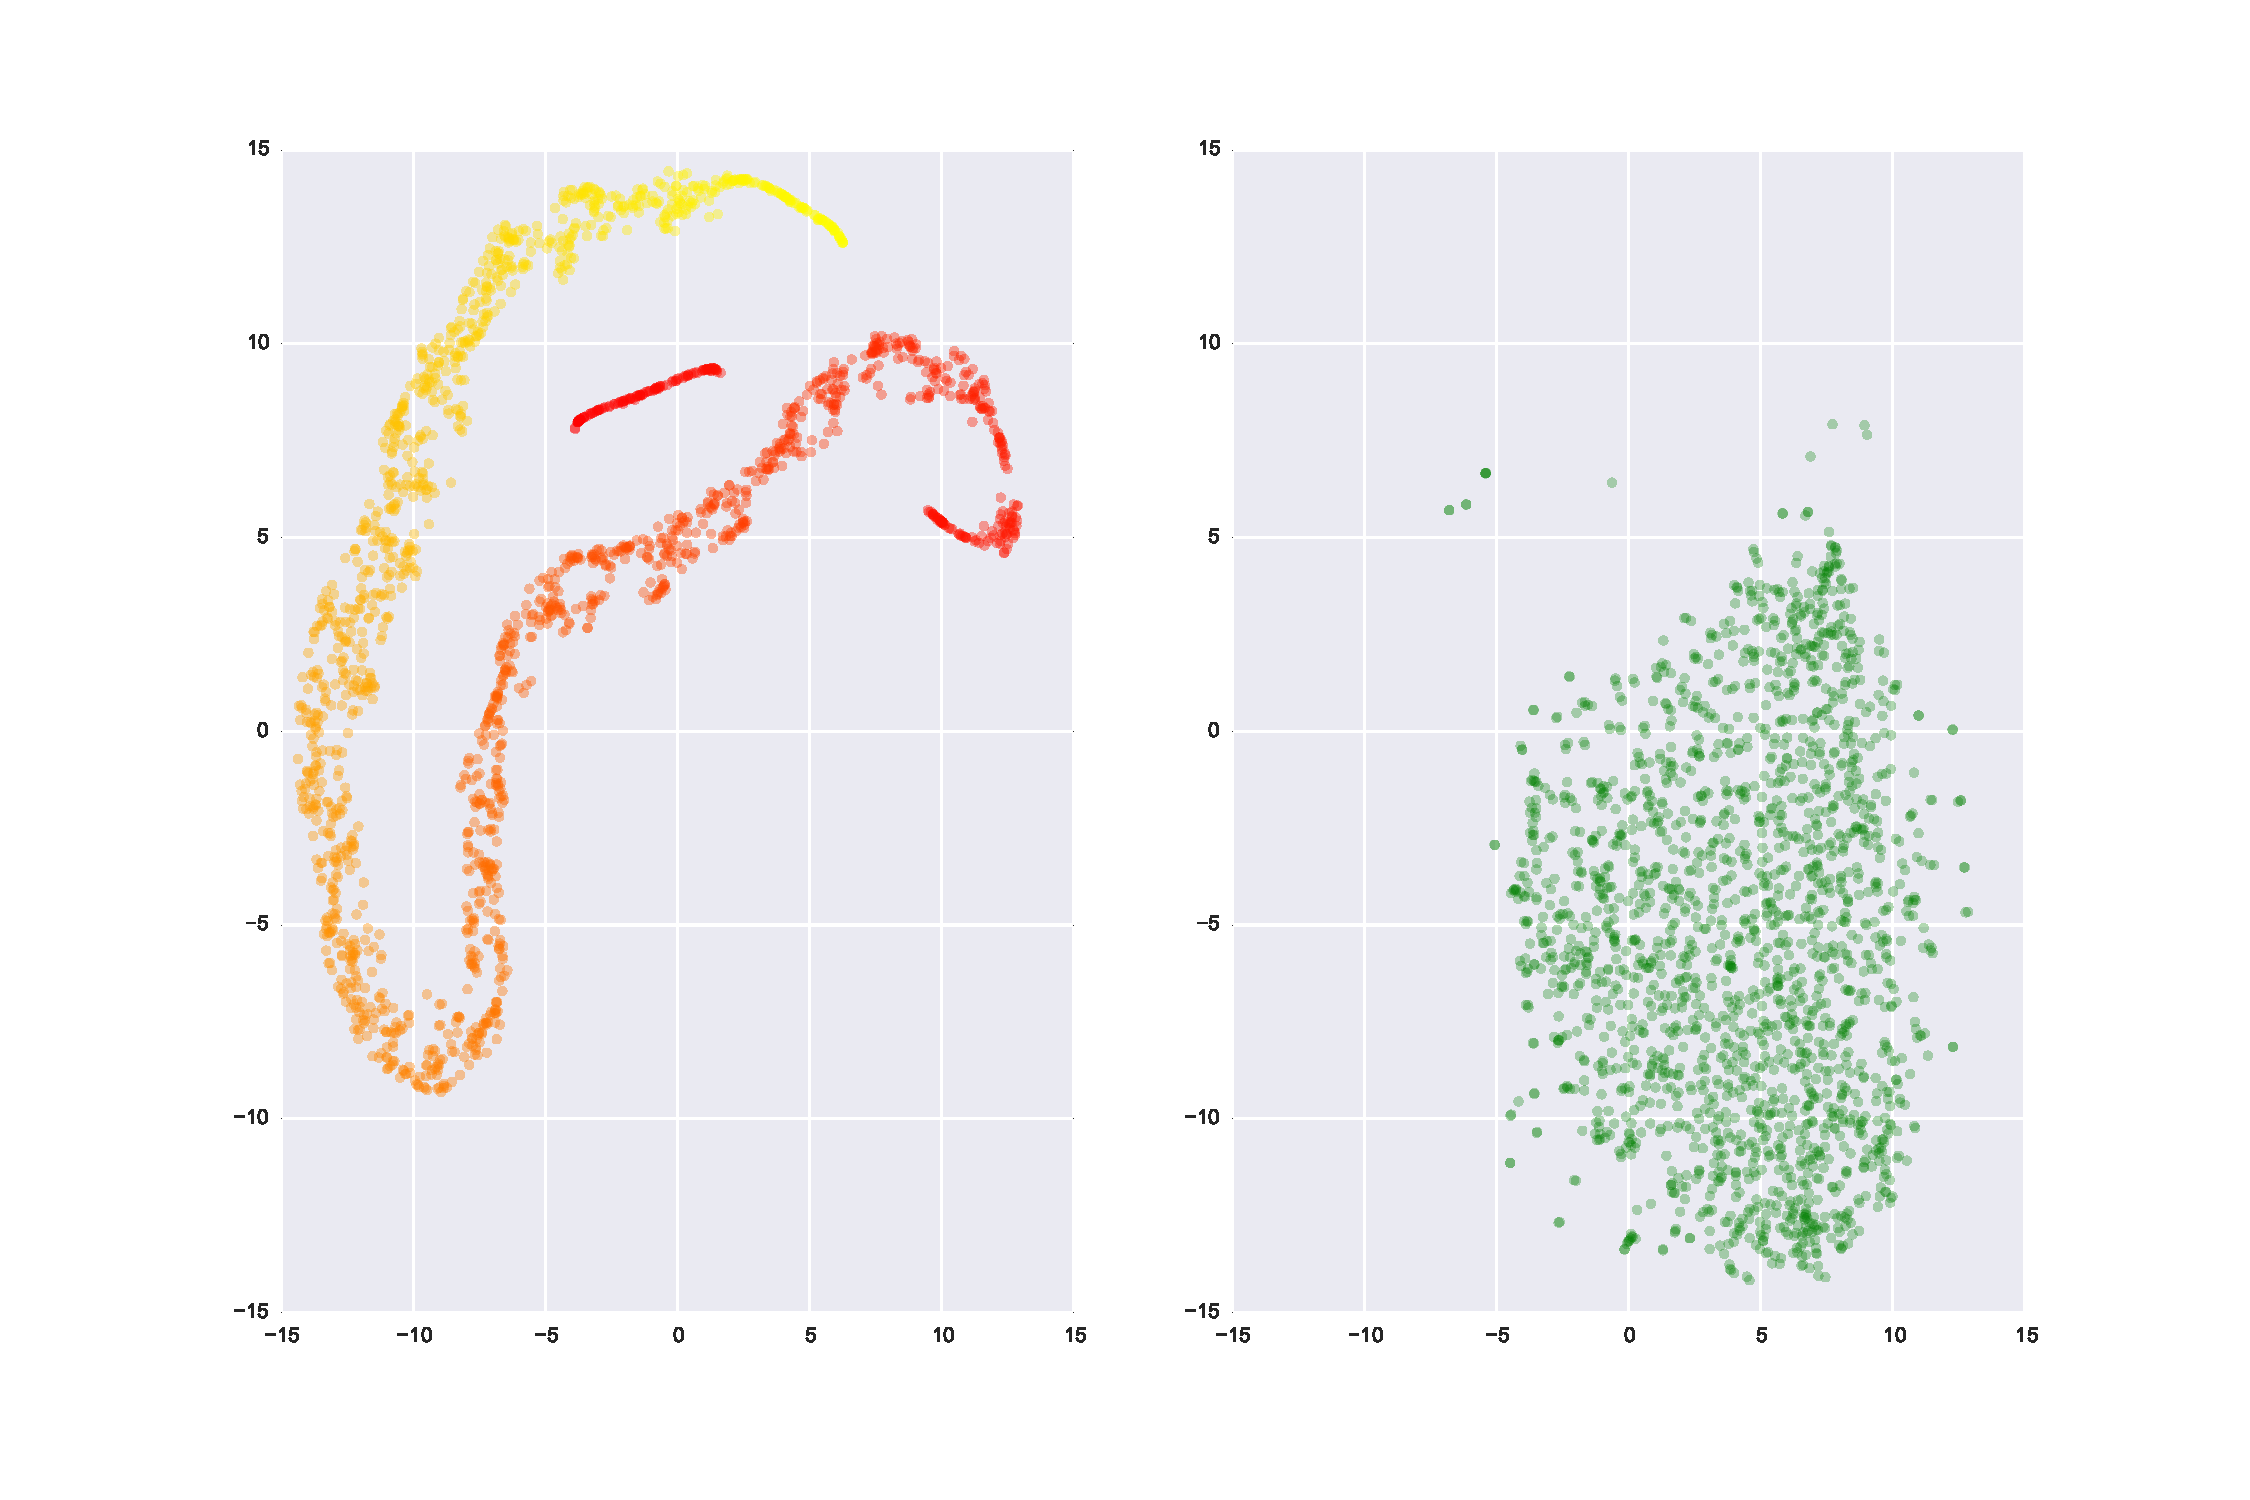
\includegraphics[width=18cm]{att1.pdf}
    \caption{2-D projection of image features for the attribute \textit{Dark Hair} of the LFW10 dataset. Figure on the right represent the projection of features from the VGG-16 network. Figure on the left represents the 2-D projections of the image features from RankNet. The change in color reflects the change in the ranking strength of the attribute.}
    \label{fig:tsne_lfw_att1}
\end{figure*}

Figures \ref{fig:tsne_lfw_att0} and \ref{fig:tsne_lfw_att1} show that images are projected into a dense sub-cluster when their representations from the pre-trained VGG-16 network are projected into 2-D space. However, after fine-tuning the network with respect to the given attribute, the feature representations of the network change such that image representations are projected onto a low-dimensional manifold that exhibits interesting features. It can be seen from the image that not only images are projected onto a low-dimensional manifold (in this case a curve), but also images are ordered in this curve according to their strength of attribute.

{\small
\bibliographystyle{ieee}
\bibliography{refs}
}

\end{document}
